\section{Formation control + motoroplysninger}
\head{This section will give a short introduction to formation control in general followed by some of the individual assignments which needs to be determined before the process of design can be started.}

The theory of formation control in general is widely applied. It can be applied in assignments regarding control of robots which needs to be placed relative to each other. Depending on the given task of the robots, and which type of robots are in focus, the formation can be utilized in different ways. The robots can also be of various types: Swarm robots, driving vehicles, helicopters, aeroplanes, ships etc. which can both be manned and unmanned. The tasks that these robots needs to fulfill can vary a lot and be both as individuals in a formation or as a whole group. Swarm robots in general got many purposes such as vacuum cleaning robots, who needs to clean a rather large area or flying robots like quadcoptors who can make different kinds of assignments. When these quadcoptors work as a combined group they could lift a certain amount of payload to achieve their goal as a group, or they could work individually in a network to do several smaller tasks. An example of how quadcoptors are working together can be examined at \citep{ethswarm}.

Within the scope of this project the robots will be unmanned ships, \ac{ASV}. The ship's main purpose will be to map the sea bed by using sonars. When one ship need to do this alone, and due to the range of the sonar, the time spend could be improved. The sonar scanning would be done as seen on figure \missingfigure{Billede af enkelt baad som anvender sonar til at scanne havbund}. When only one ship need to map a complete sea bed this process could take up a lot of time dependent on the area that need to be covered. The time spend could be improved to make this mapping more efficient. One way of optimizing the time used is to add more ships to help map the sea bed. To make the process of this as optimal as possible it could be of benefit to implement formation control in the specific assignment. This could be done in several ways, but is mostly thought of in a rigid formation, such that the formation maps the same area of the sea bed the whole time. The idea can be seen on figure \missingfigure{Billede af flere baade som anvender sonar til at scanne havbunden}. The distances between the ships would be determined by how far the sonars could reach the sea bed. There should be some overlap of the maps from each sonar but still as little as possible. The specific formation could be a simple line or it could be more advanced formations. This does not have any relevant impact of how the mappings of the sea bed would be due to the subsequent processing of the collected data from the maps. Different formations of ships can be seen on figure \ref{fig:diffforms}.
\begin{figure}[htbp]
	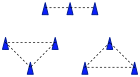
\includegraphics[width=0.5\textwidth]{fig/diffforms}
	\caption{Different formations which the \ac{ASV}s can make.}
	\label{fig:diffforms}
\end{figure}

\subsection{Considerations of formation control}
When doing formation control it is important to figure out what one
want to achieve, and depending on the strategy and the formation type
some things are to be considered as requirements regarding how the
formation should work. We are considering lawnmower patterns in this
discussion. In this work two ships are considered for simplicity, but
it should be extensible to n-number of ships.

When starting the mission, the ships may start at positions that
is not in the desired formation, it is important that the ships are in
formation when they start tracking the desired track. Therefor some
attention must be given on how to make the ships initialize this
formation. An approach is to make the ships sail individually to the
starting positions with a speed that makes them hit their respectively starting points at
the same time. If one reaches its start point much earlier
than the other it must stop, which is not wanted because it then can
drift out of position again. This basically means that there is a
tracking phase and an initialization phase. The start heading should of
course align with the path at that point.

Another issue to be considered is to ensure that no ship at
any point in time reaches a minimum speed that is necessary for the
ship to not drift out of formation. This could be a problem in corners
of the formation if a stiff construction, where the inner most ship
has to move slower, to accommodate the shorter distance on an inner
circle arc.

Faults like blackout on a ship could also be considered in the control
design. I.e. what happens with the formation when one ship faults in a
blackout. Should the rest of the formation stop, should the formation
still follow this drifting ship or should the mission simply terminate
when it is discovered that a ship has blackout.

In the initialization phase it is also relevant to consider how the
ships should avoid each other if they are on the wrong side of each
other.

\begin{figure}[htbp]
	\centering
	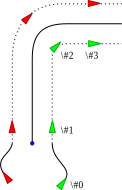
\includegraphics[width=0.8\textwidth]{fig/cornoring}
	\caption{Two ships initializing and following the path offset
		equally on each side, ships are constrained to sailing parallel
		and heading the same as path when projected onto the path. Blue
	dot is start of path. Fully drawn splines is initializing phase.}
	\label{fig:cornoring}
\end{figure}

On figure~\vref{fig:cornoring} is a simple path following performed
with two ships in a stiff formation with an equal distance from the
path. It illustrates four steps, in step \#0 the ships initializes a
random position near the start of the path. At \#1 it is tracking the
path in formation, whilst still in formation. At \#2, the green
(right) ship is in a tight inner curve where it is important to
consider design of the path such that the capabilities of the ship is not
exceeded to stay in formation. At \#3 it is back to straight line path
following in formation.


\subsubsection{Degree of Actuation}
The degree of actuation is a matter that sets some limitations on how
the path following can be made, and thus the methods available to
control the ships.

AAUSHIP is a ship, which means that is is not fully actuated in the
whole 3D space, but this is not needed since it is moving on a
surface. To be fully actuated it must be able to have controls for
surge, sway and yaw.

\todo{State if it is fully actuated in this sense}